\section{Experiments}
\label{sec:experiments}
We perform all our experiments using our collected dataset, and evaluate multiple system settings for pose and segment to validate each component.
For obtaining GPS and IMU signal, due to at each time step, one sampled noisy signal can obtained. This is limited for training the system. Thus, follow~\cite{vishal2015accurate}, we simulate GPS and IMU error by adding random noise $\epsilon$ with uniform distribution. Specifically, translation and rotation noise are set as $\epsilon_t \sim U(0, 7.5)$ and rotation $\epsilon_r \sim U(0^{\circ}, 15^{\circ})$ respectively. We refer to realistic data~\cite{lee2015gps} for setting range of simulation noise.

In this paper, our data vehicle collected 6 videos at different daytimes surrounding a technology park. The 3D map generated in our experiment has a road length around 3500$m$, and the distance between consecutive frames is around 5$m$ to 10$m$. We use 4 of the videos for training and 2 for testing, yielding 2242 training images and 756 testing images. The semantic classes included in the dataset includes $\{$sky, car-lane, ped-lane, bike-lane, curb, traffic-cone, traffic-stack, traffic-fence, light-pole, traffic-light, tele-pole, traffic-sign, billboard, building, security-stand, plants, object $\}$. In the future, we are targeting at constructing even larger datasets with more semantics.

\paragraph{Implementation details.} To quickly render from the 3D map, we adopt OpenGL to efficiently render a label map while handling the z-buffer operation. A 512 $\times$ 608 image can be generated in 70ms with a single Titan Z GPU, which is also the input size for both pose network and segment network. For segment output, we keep the size the same as input. Both of the network is learned with 'Nadam' optimizer~\cite{dozat2016incorporating} with a learning rate $10^{-3}$. For training pose RNN, we sample a video sequence with 100 frames from the training data. We sequentially train the three models due to GPU memory limitation.
For pose CNN and segment CNN, we stops at 100 epochs, and for pose RNN, we stops at 200 epochs. For data augmentation, we use the imgaug\footnote{https://github.com/aleju/imgaug} library to variate lighting, blurring and flipping. We select a subset from training images for validation trained model from each epoch, and choose the model performing best for evaluation.

For testing, to get a confidence range for the prediction for verifying the effectiveness of each model, we report the standard variation of the results from a 10 time simulation. Finally, we implement all the networks by adopting the MXNet~\cite{ChenLLLWWXXZZ15} platform.


\paragraph{Pose Evaluation.}
In \tabref{tbl:pose}, we show the pose estimated results. We first direct following the work of PoseNet~\cite{Kendall_2015_ICCV,kendall2017geometric}, and use their published code to train a model. Due to scene appearance similarity of the street-view (\figref{fig:data}), it does not give reasonable results, \ie better than the noisy GPS and IMU signal, in our experiments.
By using only CNN and coarse pose prior, the model can start to learn reasonable relative poses (3rd row), which significantly reduces the pose error. When inserting semantic cues such as road priori and semantic weights in \equref{eq:proj_loss}, the pose results is significantly improved, especially at rotation (4th row).
Finally, RNN gives strong cues about the moving speed and acceleration of the camera, yields the best results for both translation and rotation.

\begin{table}
\center
\fontsize{8}{9}\selectfont
\begin{tabular}{lccc}
\toprule[0.1 em]
% \thickhline
Method & Trans (m) & Rot ($\circ$) & Pix. Acc($\%$)\\
\hline
PoseNet~\cite{kendall2017geometric} & -  & -  & -  \\
$\xi$ pose & 3.45 $\pm$ 0.076 & 7.87 $\pm$ 0.10 & 54.01 $\pm$ 0.5 \\
Pose RNN w/o CNN & 1.282 $\pm$ 0.061  & 1.731 $\pm$ 0.06 &  68.1 $\pm$ 0.32 \\
Pose CNN w/o semantic & 1.355 $\pm$ 0.052  & 0.982 $\pm$ 0.023 & 70.99 $\pm$ 0.18 \\
Pose CNN w semantic & 1.331 $\pm$ 0.057  & 0.727 $\pm$ 0.018 & 71.73 $\pm$ 0.18  \\
Pose CNN w KF & 1.281 $\pm$ 0.06  & 0.833 $\pm$ 0.01 &   \\
Pose CNN-RNN  & \textbf{1.005} $\pm$ 0.044  & \textbf{0.719} $\pm$ 0.035  & \textbf{73.01} $\pm$ 0.16  \\
\toprule[0.1 em]
\end{tabular}
\caption{Compare the accuracy of different settings for pose estimation.
$\xi$ pose indicates the input signal from GPS, IMU.
The number after $\pm$ indicates the std from 10 simulations. We can see the improvement is statistically significant.}
\label{tbl:pose}
\vspace{-0.3\baselineskip}
\end{table}

\begin{figure*}
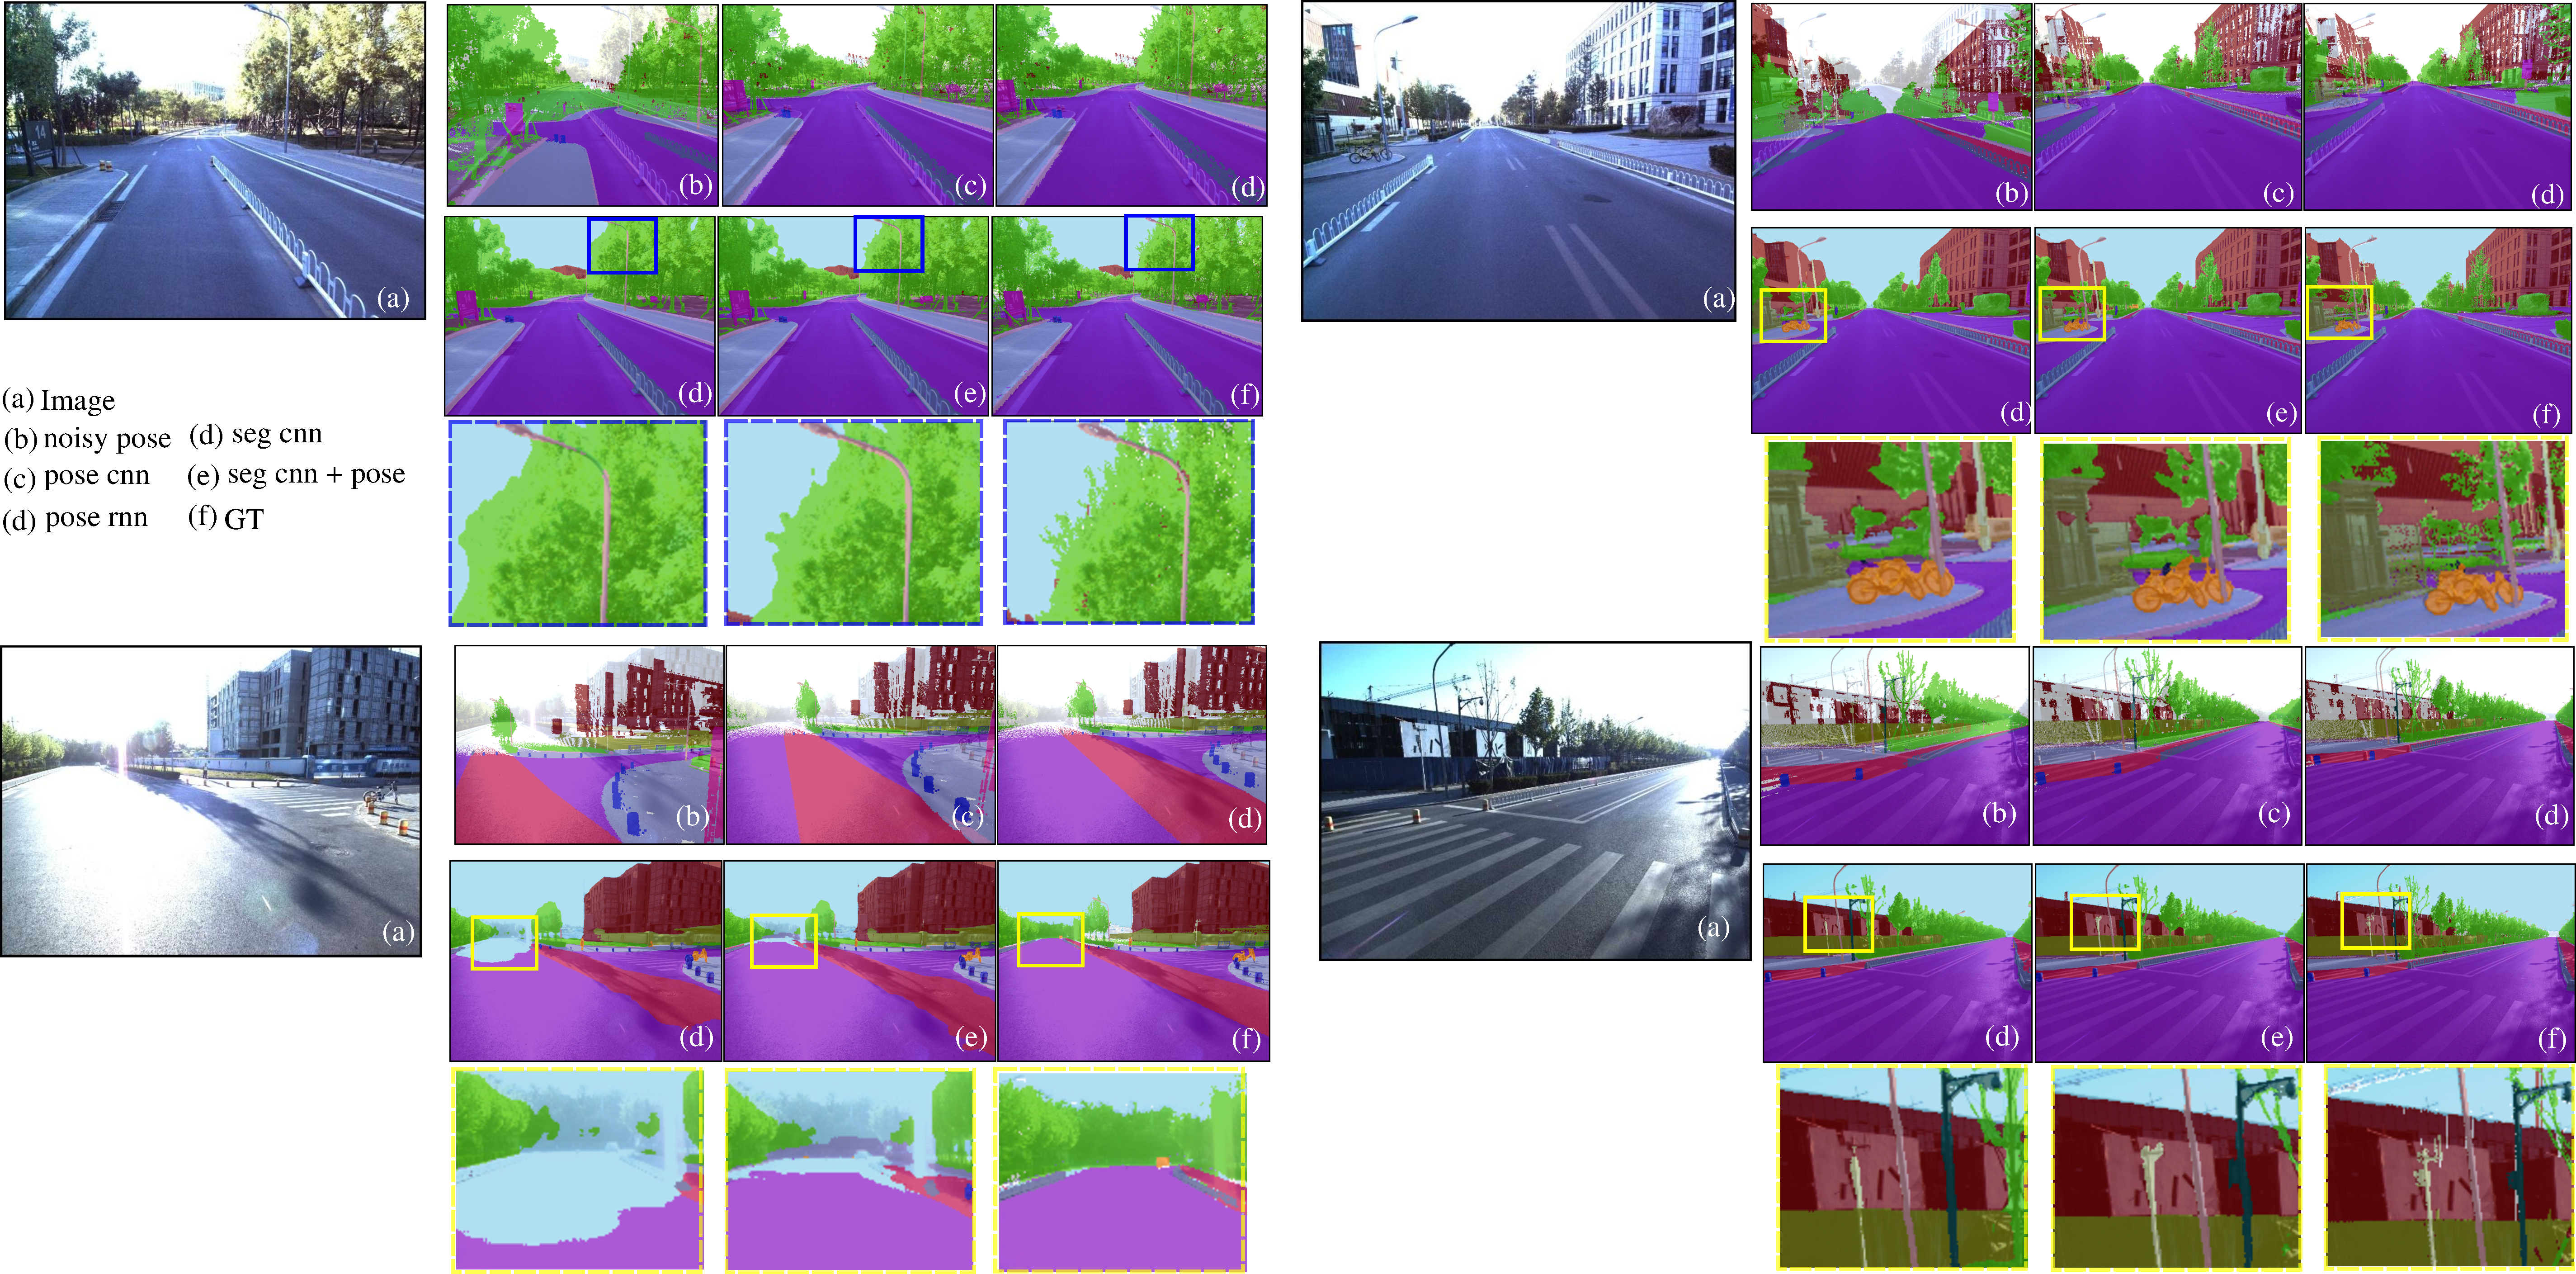
\includegraphics[width=\textwidth]{fig/results.pdf}
   \caption{Results from each intermediate stage out of the system. We indicate the }
\label{fig:results}
\vspace{-0.8\baselineskip}
\end{figure*}

\paragraph{Segment Evaluation.}
In \tabref{tbl:segment}, we show the scene parsing results. We first use one of the state-of-the-art parsing network on the CityScapes \ie ResNet38~\cite{WuSH16e}. It has pre-trained parameters from both ImageNet and CityScapes, running with a 5s per-frame with our resolution. Although the results could be good, it is too slow for real-applications. Our network can run in 0.1s, while yields comparable results (4th row). At 2nd row, we use the ground truth pose to obtain an upper-bound for the segmentation performance. In this case, the projected label map aligns perfect with the image, thus yields significantly better results than the rest. At 3rd row, we train the segment network without pose prior.  Notice that for a fair comparison, after convergence at 100 epoch, we continue train the network another 100 epochs in order to avoid the influence from longer training.
At 4th and 5th row, we show the results train with rendered label map from pose CNN and pose CNN-RNN respectively, where better pose can help the segment accuracy get closer to the oracle case, which demonstrate the effectiveness of our strategy. Due to space limit, we leave per-class results to the supplementary.

% \begin{table*}
% \center
% \fontsize{6}{7}\selectfont
% \begin{tabular}{lcccccccccccccccccc}
% \toprule[0.1 em]
% %\thickhline
% Method & mean IOU & sky & car-lane & ped-lane & bike-lane & curb & $t$-cone & $t$-stack & $t$-fence & light-pole & traffic-light & tele-pole & $t$-sign & billboard & building & security-stand & plants & object \\
% \hline
% ResNet38~\cite{} & & &  & & & & & & & & & & & & & & &  \\
% Segment CNN w oracle pose & & & & & & & & & & & & & & & & & &  \\
% Segment CNN w/o pose & & & & & & & & & & & & & & & & & &  \\
% Segment CNN w pose CNN & & & & & & & & & & & & & & & & & & \\
% Segment CNN w pose CNN-RNN & & & & & & & & & & & & & & & & & & \\
% \toprule[0.1 em]
% \end{tabular}
% \caption{Compare the accuracy of different segment networks setting. $t$ is short for 'traffic' in the table. $\pm$ indicates the confidence region by 10 time GPS simulation.}
% \label{tbl:segment}
% \vspace{-0.3\baselineskip}
% \end{table*}

\begin{table}
\center
\fontsize{8}{9}\selectfont
\begin{tabular}{lccc}
\toprule[0.1 em]
%\thickhline
Method &Pix. Acc ($\%$) &  mAcc ($\%$) & mIOU ($\%$) \\
\hline
ResNet38~\cite{WuSH16e} & 95.87 & 71.92 & 64.66 \\
SegCNN w pose GT & 97.1 & 86.8 & 79.37 \\
SegCNN w/o Pose & 95.61 & 77.09 & 68.35 \\
% SegCNN $\xi$ Pose & 95.63 $\pm$ 0.02 & 77.39 $\pm$ 0.21 & 68.41 $\pm$ 0.15\\
SegCNN w Pose CNN & 95.67 $\pm$ 0.01 & 77.95 $\pm$ 0.16 & 68.6 $\pm$ 0.12\\
SegCNN Final & \textbf{95.98} $\pm$ 0.004 & \textbf{79.36} $\pm$ 0.08 & \textbf{69.93} $\pm$ 0.08 \\
\toprule[0.1 em]
\end{tabular}
\caption{Compare the accuracy of different network settings. $\pm$ indicates the standard variation by 10 times GPS simulation. 
The meaning of each label map for an image is indicated by a layout map at left top. 
Full table for all class accuracy is available in our supplementary materials.}
\label{tbl:segment}
\vspace{-0.3\baselineskip}
\end{table}

\paragraph{Qualitative results.} In \figref{fig:results}, we select a subsequence composed of 5 frames to show the results. More results are provided in the supplementary material. At 2nd and 3rd column, we show how the pose network aligns the image with pose from view of camera. At 4th and 5th column, we compare the segment results taking only images as input and those also consider rendered label map. As can be seen at the circled regions, the segment results with pose rendered label maps not only give better accuracy, but also have better temporal consistency.
